\setcounter{section}{1}
\fancyfoot[R]{v1.1}

\section{Pseudosolutions}
\subsection*{Intuition behind pseudosolutions}
    \par 
    Let's recall that the system of linear equations (SLE) can be represented using the following notation
    \[
        A\vec{x} = b,
    \]
    where
    \[
        A = 
            \begin{bmatrix}
                a_{11} & \cdots & a_{1n}\\
                \vdots & \ddots & \vdots\\
                a_{m1} & \cdots & a_{mn} 
            \end{bmatrix}
        \in M_{m\times n}(\C), \quad 
        \vec{b} = \begin{bmatrix}  b_1 \\\vdots \\b_,\end{bmatrix} \in \C^m, \quad
        \vec{x} = \begin{bmatrix}  x_1 \\\vdots \\x_n\end{bmatrix} \in \C^n.
    \]
    Let's recall possible solution sets of SLE
    \begin{theorema}{Solution sets of SLE}
        A linear system of equations may behave in any one of three possible ways
        \begin{enumerate} 
            \item The system is definite - has a single unique solution.
            \item The system is indefinite - has infinitely many solutions.
            \item The system is inconsistent - has no solution.
        \end{enumerate}
    \end{theorema}
     \Ex Definite system of the square system.
    
        If $A \in M_{n\times n}(\C), \ \rank A = n$, then we can easily obtain unique solution $\vec{x}$ by inverting the matrix of initial coefficients
            \[
                \vec{x}  = A^{-1}\vec{b}.
            \]\\
    We want to generalize this result for any systems (definite, indefinite and inconsistent of any size). Let's outline intuition of this generalization in the following examples.
\subsubsection*{Definite system}
    \Ex If $A \in M_{m\times n}(\C), \rank A=n$, then there exist unique solution $\vec{x}$. For example, consider a system 
        \begin{wrapfigure}[15]{r}{0.4\columnwidth}
            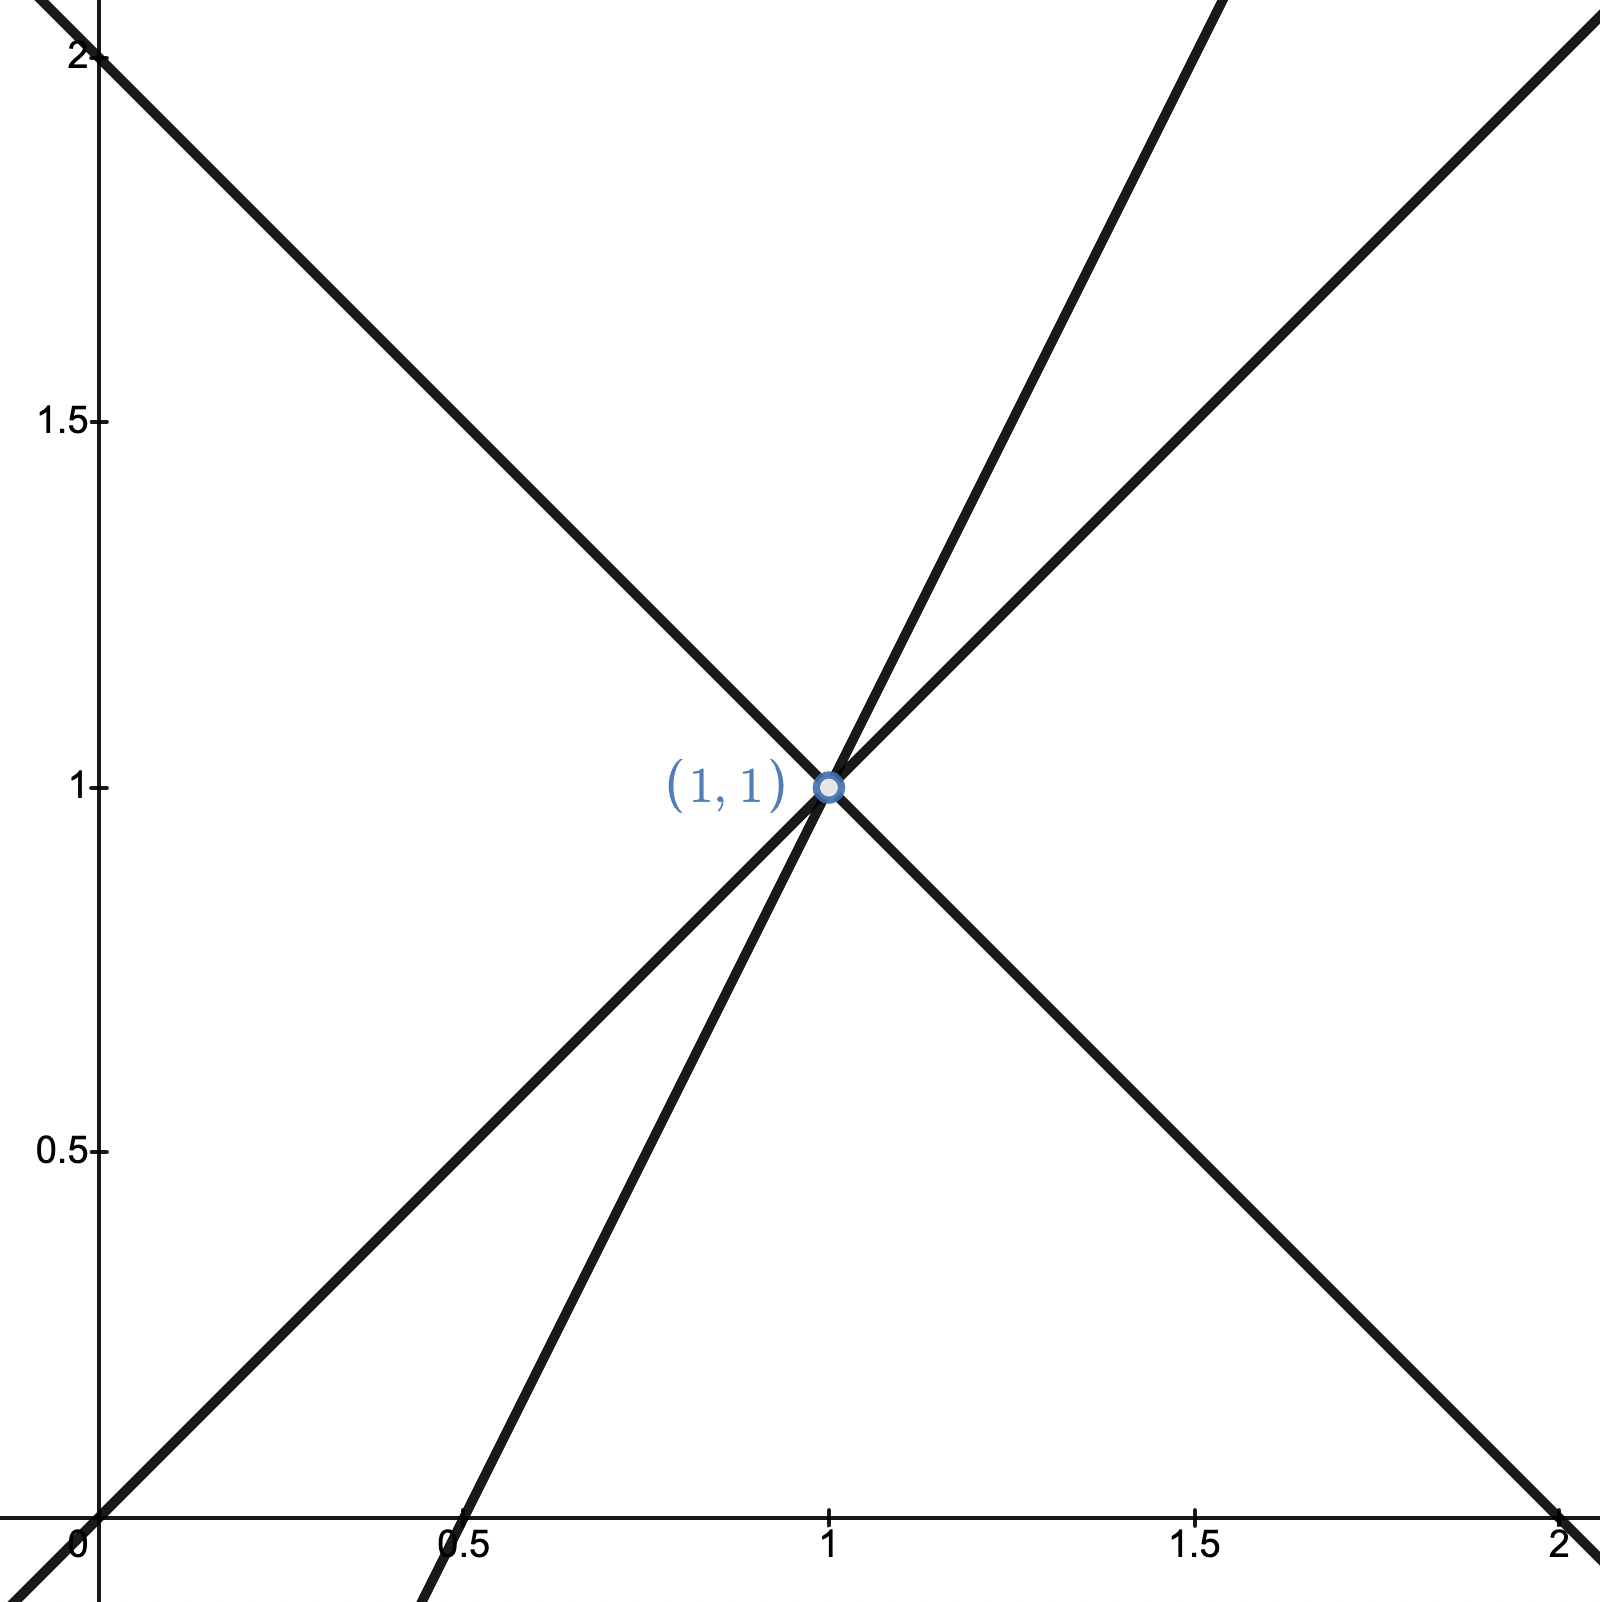
\includegraphics[width=0.4\columnwidth]{lectures/images/definite_system.png}
            \caption*{\scriptsize{Example of definite system.}}
            \label{fig:definite_system}
        \end{wrapfigure}
        \[
            \left\{
                \begin{array}{l}
                    x-y = 0\\
                    x+y = 2\\
                    2x-y = 1
                \end{array}.
            \right.  
        \]
        The system has only one solution in the point $\vec{x} = \begin{bmatrix}1\\ 1\end{bmatrix}$. However, we would like to generalize the method of obtaining a solution in such a way that it looks similar to the first example (definite system of square system)
        \[
            \vec{x} = ?\cdot \vec{b}.  
        \]
    
        And looking ahead we can obtain such a factor to express solution that way. But now let's get a broader generalization.\newpage

\subsubsection*{Indefinite system}
    \Ex Consider a system~~~~~~~~~~~~~~~~~~~~~~~~~~~~~~~~~~~~~~~
    \begin{wrapfigure}[15]{r}{0.4\columnwidth}
        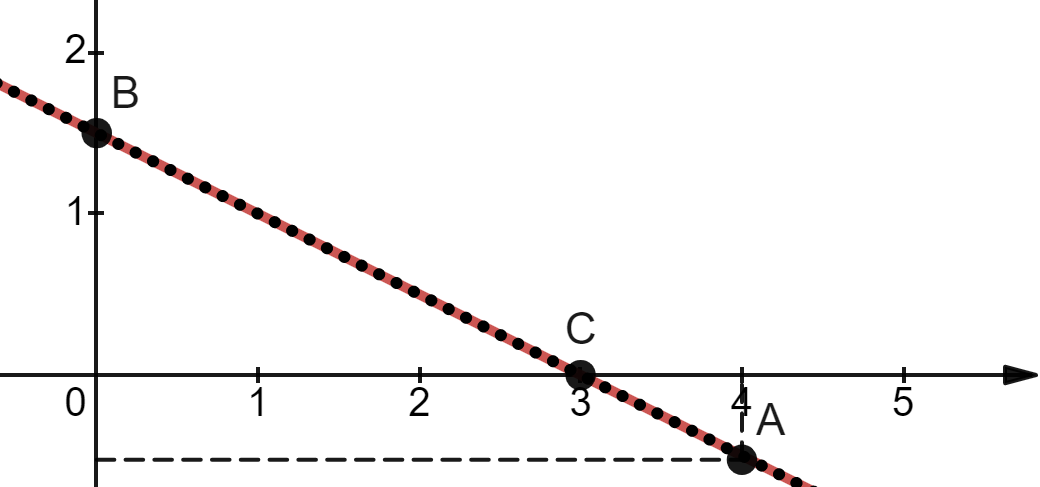
\includegraphics[height=0.4\columnwidth, width=0.4\columnwidth]{lectures/images/indefinite_system.png}
        \caption*{\scriptsize{Example of indefinite system.}}
    \end{wrapfigure}
    \[
        \left\{
            \begin{array}{l}
                2x-y=1\\
                4x-2y=2
            \end{array}.
        \right.  
    \]
    It is not so obvious to choose a specific solution here because a whole family of solutions of the following form 
    $\vec{x} = 
    \begin{bmatrix}
        x\\1-2x
    \end{bmatrix}$ is suitable for us. At the same time, we would like express solution of the system in the following form
    \[
        \vec{x} = ?\cdot \vec{b},
    \]
    which assumes one solution, not infinite. For this reason, we need to choose the best solution out of infinite. In other words, we need to define "optimal" solution. Our intuition hints us to a solution point which is the closest to the origin. \\\\\\\\
    

\subsubsection*{Inconsistent system}    
     \Ex Consider a system~~~~~~~~~~~~~~~~~~~~~~~~~~~~~~~~~~~~~~~
        \begin{wrapfigure}[8]{r}{0.4\columnwidth}
            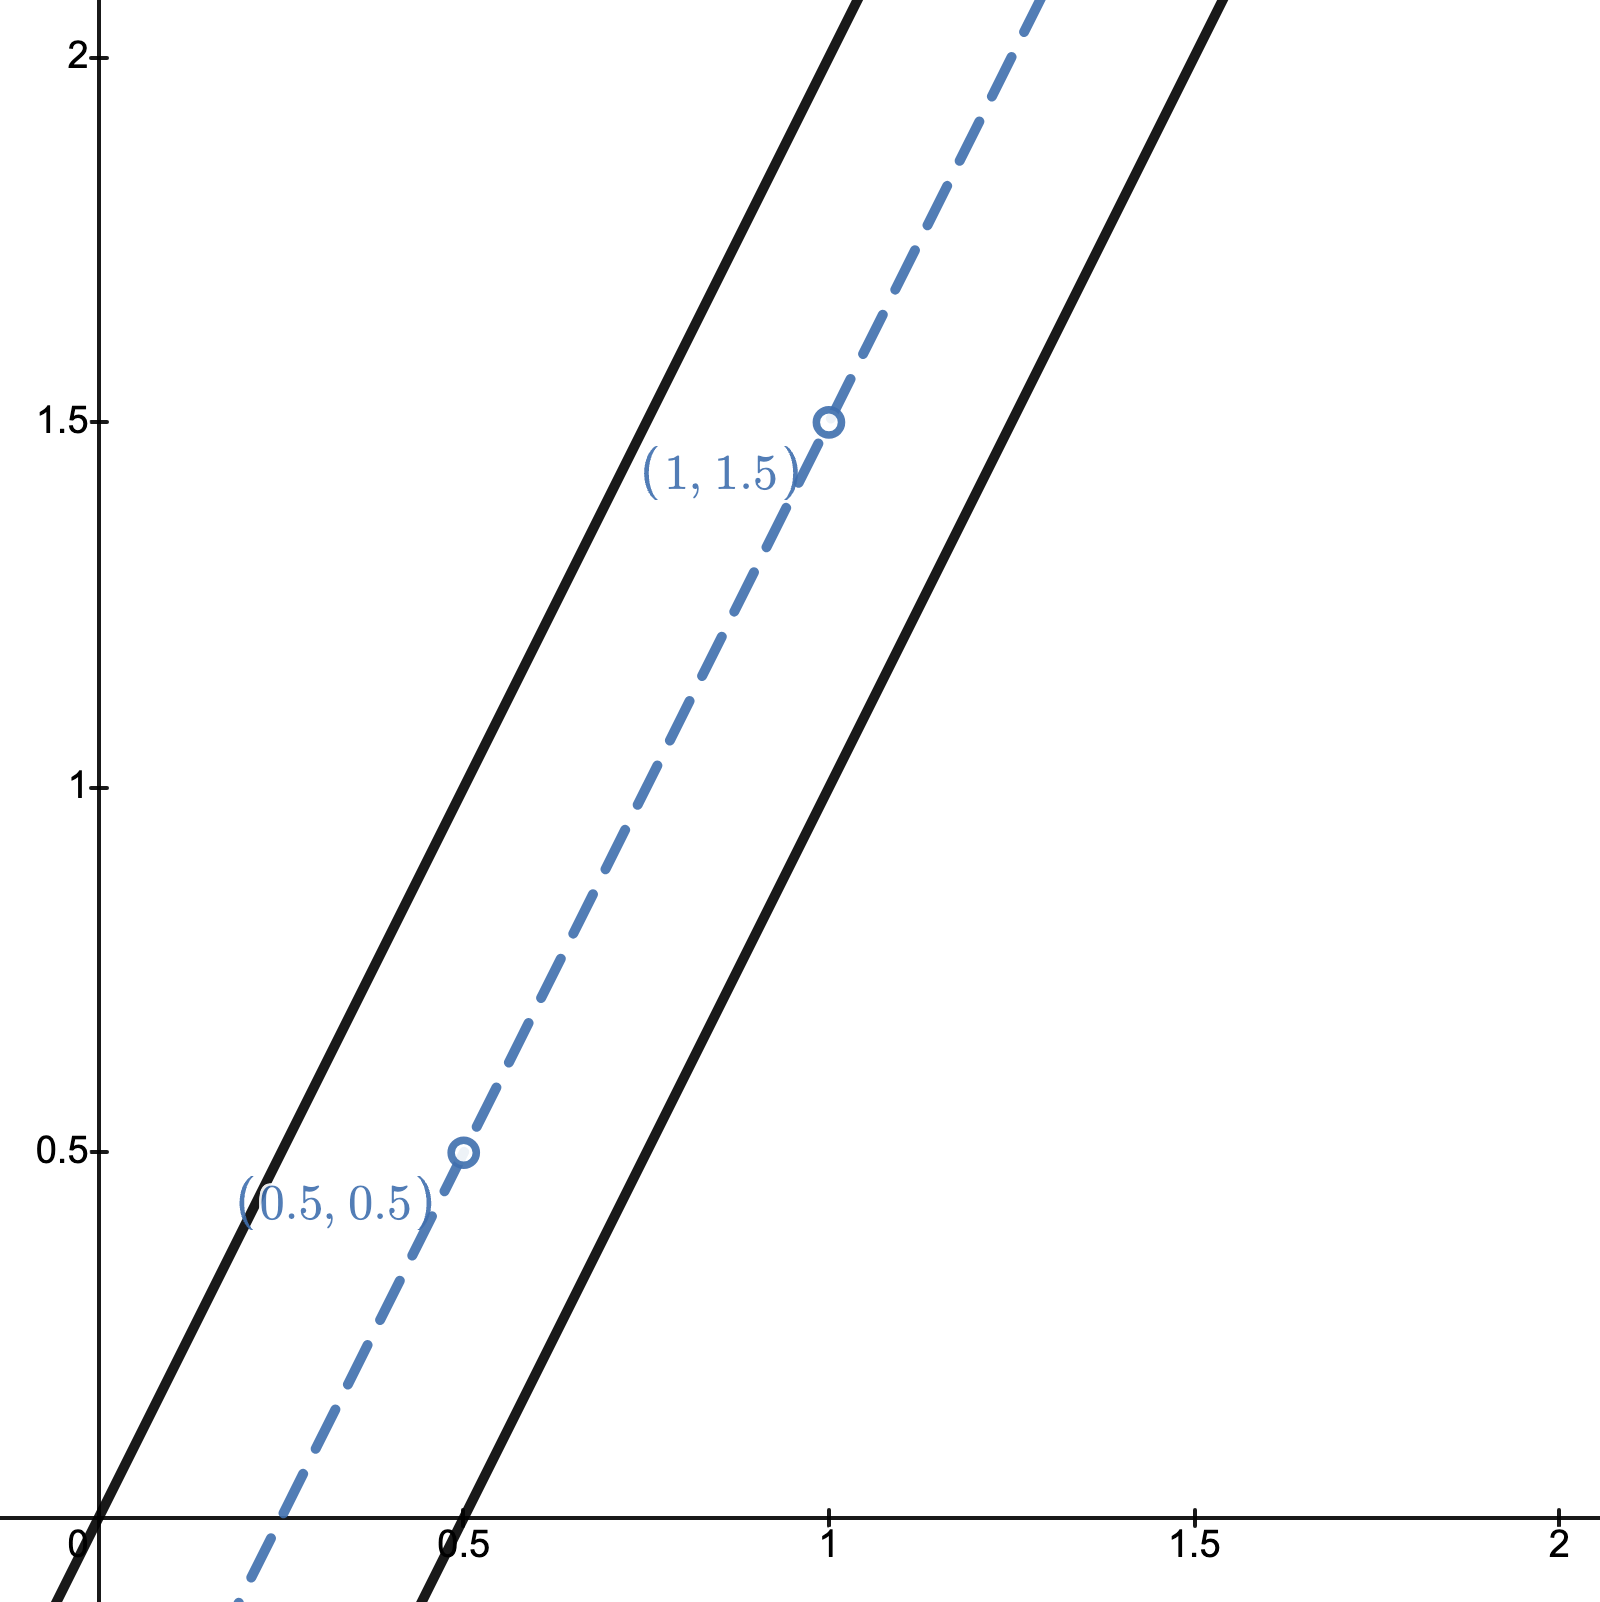
\includegraphics[width=0.4\columnwidth]{lectures/images/inconsistent_system.png}
            \caption*{\scriptsize{Example of inconsistent system.}}
            \label{fig:inconsistent_with_vectors}
        \end{wrapfigure}  
        $$
            \left\{
                \begin{array}{c}
                    2x-y=0,\\
                    2x-y=1
                \end{array}.
            \right.  
        $$
        The system does not have solution. Geometrically the system describes two parallel lines. Our intuition hints us to choose a point on a line right in middle of the parallel lines. However, it is still a whole family of solutions that can be the answer to the request of the product or business problem. 
        \newpage
\subsection*{Pseudosolution}
    \begin{definition}{Pseudosolution}{}
        Consider a system of a linear equations $A\vec{x} = \vec{b}$. A vector $\vec{u} \in \C^n$ is called a pseudosolution (or least square solution), if
        \[
            \left| A\vec{x} - \vec{b} \right| \ge \left| A\vec{u} - \vec{b} \right|,
            \quad
            \forall \vec{x} \in \C^n. 
        \]
        That is, vector $f(\vec{x}) =\begin{bmatrix}f_1\\ \vdots\\f_n\end{bmatrix}= A\vec{x}-\vec{b}$ reaches it's minimum length at $\vec{x}=\vec{u}$. That is, $\vec{x}=\vec{u}$ is the solution of the following problem
        $$|f(x)|^2 = |f_1|^2 + \ldots + |f_n|^2 \rightarrow \mathop{min}_{\vec{x}}.$$ 
    \end{definition}
    \begin{theorema}{$\vec{u} := A^+\vec{b}$}{}
        The vector $\vec{u} = A^+\vec{b}$ is a pseudosolution of the system of linear equations $A\vec{x} = \vec{b}$. Moreover, among all pseudosolutions, the vector $\vec{u}$ is the unique pseudosolution with minimal length.
    \end{theorema}
    \begin{proposition}{}{}
        If $\hat{x}$ is a solution, then it is a pseudosolution.
    \end{proposition}
    \begin{proof}
        $A\hat{x} - \vec{b} = 0 \Longrightarrow \left| A\hat{x} - \vec{b} \right| = 0 = \min |f_x|^2.$
    \end{proof}
    \vspace*{0.2cm}
    \begin{proposition}{1}{}
        \begin{tabular}{|l|l|}
            \hline
            Type of a system & Solution \\ \hline
            definite         &      $\hat{x}=A^+\vec{b}$  is the solution  \\ \hline
            indefinite       &   $\hat{x}=A^+\vec{b}$  is the solution of minimal length       \\ \hline
            inconsistent     &    $\hat{x}=A^+\vec{b}$  is the pseudosolution  of minimal length    \\ \hline
        \end{tabular}
    \end{proposition}
    \begin{lemma}{1}{}
        $\im (AA^+-I) \perp \im (A) $.
    \end{lemma}
    \begin{proof}    
        Let us denote $ AA^+-I$ by $M$. Let us denote vector columns that generate $\im(M)$ and $\im(A)$ by $M^i$ and $A^j$ respectively. Then the following holds
        \begin{eqnarray}
            &&\im(M)  \perp \im (A) \label{1}\\
            \Leftrightarrow &&M^i \perp A^j,\quad \forall i,j\nonumber\\
            \Leftrightarrow &&(M^i, A^j)=0,\quad \forall i,j\nonumber\\
            \Leftrightarrow &&(M^i)^*\cdot A^j=0,\quad \forall i,j\nonumber\\
            \Leftrightarrow &&M^*A=0,\label{2}
        \end{eqnarray}
        which means that by proving (\ref{2}), we get (\ref{1}). Let us prove (\ref{2}).
        \begin{eqnarray}
            &&M^* A=(AA^+-I)^* A
            =((AA^+)^*-I^*)A 
            =(AA^+)^*A-I^* A
            \stackrel{\text{axiom III}}{=}AA^+A-I
            \stackrel{\text{axiom I}}{=}A-A=0\nonumber.
        \end{eqnarray}
    \end{proof}
    \begin{theorema}{Pythagoras}{}
        Suppose $\vec{a} \perp \vec{b}$, then for $\vec{c} = \vec{a} + \vec{b}$, we have $|\vec{c}|^2 = |\vec{a}|^2 + |\vec{b}|^2.$ In particular $|\vec{c}| \geq |\vec{b}|$. The equality holds only for $\vec{a} = \vec{0}$.
    \end{theorema}      
    \begin{proof}
        We leave as an exercise for the reader.
    \end{proof}
    \begin{proof}(of Theorem $\vec{u} = A^+\vec{b}$)~ ~ ~ ~ ~ ~ ~~ ~ ~ ~ ~ ~ ~~ ~ ~ ~ ~ ~ ~~ ~ ~ ~ ~ ~ ~~ ~ ~ ~ ~ ~ ~~ ~ ~ ~ ~ ~ ~~ ~ ~ ~ ~ ~ ~~ ~ ~ ~ ~ ~ ~~ ~ ~ ~ ~ ~ ~
        First, let us prove that $\vec{u} = A^+\vec{b}$ is a pseudosolution. Let us denote
        $$
            \vec{A}_x:= A(\vec{x}-\vec{u})=A\vec{x}-A\vec{u}\in \C^n,\quad
            \vec{B}  := (AA^+-I)\vec{b}  = A\vec{u}-\vec{b}\in \C^n,\quad
            \vec{C}  := \vec{A}_x+\vec{B} =A\vec{x}-\vec{b}.
        $$
        
         Using Lemma, we get $\vec{A}_x\perp\vec{B}$. Using Pythagoras theorem, we get
         \begin{eqnarray}
            |C|&\ge&|B|\nonumber\\
            &\Leftrightarrow&\nonumber\\ 
            |A\vec{x}-\vec{b}|&\ge&|A\vec{u}-\vec{b}|,\quad \forall \vec{x}\in \C^n,\nonumber
         \end{eqnarray}
         which means that $\vec{u}$ is a pseudosolution.
    
        Secondly, let us prove that $\vec{u} = A^+\vec{b}$ is the unique pseudosolution with minimal length.  Let us denote $w:=\vec{x}-\vec{u}$. Suppose $\vec{x}$ is another pseudosolution, which means that 
        \begin{eqnarray}   
            A\vec{x}=A\vec{u}
            \Leftrightarrow A(\vec{x}-\vec{u})=0
            \Leftrightarrow Aw=0.\label{aw}
        \end{eqnarray}
        Let us consider the following
        \begin{eqnarray}
          \left(\vec{u}, \vec{w}\right) 
          &=& \vec{u}^* \vec{w} 
          = (A^+\vec{b})^* \vec{w} 
          = \vec{b}^*A^{+^*} \vec{w}\nonumber\\
          &\overset{\rom{2}}{=}& \vec{b}^*\left(A^+AA^+\right)^*\vec{w}  
          = \vec{b}^*A^{+^*}\left(A^+A\right)^*\vec{w}  \nonumber\\
          &\overset{\rom{4}}{=}& \vec{b}^*A^{+^*}A^+A\vec{w}\nonumber\\
          &=&\vec{b}^*A^{+^*}A^+
        \overset{(\ref{aw})}{=} 0,\nonumber
    \end{eqnarray} 
        which means that $u\perp w$. Using Pythagoras theorem, we get $|\vec{x}|\ge|\vec{u}|$, which means that $\vec{u}$ is pseudosolution with minimal length. By Pythagoras theorem $|\vec{x}|=|\vec{u}|\Leftrightarrow\vec{w}=0\Leftrightarrow \vec{x}=\vec{u}$, which means that $\vec{u}$ is unique.
    \end{proof}
    \begin{problem}{Finding a pseudosolution}
        Find a pseudosolution of the following inconsistent system
        \[
            A = \begin{bmatrix}
                2 & 1\\
                2 & 1
            \end{bmatrix}, \hspace*{0.5cm} \vec{b} = \begin{bmatrix}
                3 \\ 6
            \end{bmatrix}.  
        \]
        \begin{solution}
            Then pseudosolution can be found by the formula
            \[
                \vec{u} = A^+\vec{b}.  
            \]
            Since $\rank(A)=1$, we could apply following formula for pseudoinverse of matrix $A$ 
            \[
                A^+ = \dfrac{1}{\sum{a_{ij}^2}} A^* 
                = \dfrac{1}{1^2+1^2+2^2+2^2} 
                \begin{bmatrix}
                    2 & 1 \\
                    2 & 1
                \end{bmatrix}^* 
                = \dfrac{1}{10} 
                \begin{bmatrix}
                    2 & 2 \\
                    1 & 1
                \end{bmatrix}.
            \]
            Finally, we get a pseudosolution of the system
            \[
                \vec{u} = \dfrac{1}{10} \begin{bmatrix}
                    2 & 2 \\
                    1 & 1
                \end{bmatrix} \cdot \begin{bmatrix}
                    3 \\ 
                    6
                \end{bmatrix} = \dfrac{1}{10} \begin{bmatrix}
                    18 & 9
                \end{bmatrix}.
            \]
        \end{solution}
    \end{problem}
    
    \begin{lemma}{2}{} 
        $$
            A\vec{x}=\vec{b}
            \quad
            \Leftrightarrow
            \quad
            A\vec{x}=AA^+\vec{b}.
        $$
    \end{lemma}
    \begin{proposition}{}{}
        $\vec{x}$ is a pseudosolution
        $\Leftrightarrow
        \vec{x}$ is a solution of the ''normal system'', which means
        \[  
            A\vec{x}=\vec{b}
            \quad
            \Leftrightarrow
            \quad
            A^*A\vec{x} = A^*\vec{b}.  
        \]
    \end{proposition}
    \begin{proof}
        Let $\vec{x}$ be a pseudosolution of the system $A\vec{x}=\vec{b}$. Let us prove that pseudosolution $\vec{x}$  is also a solution the normal system $A^*A\vec{x} = A^*\vec{b}$
        \begin{eqnarray}    
            A^*A\vec{x}
            &\stackrel{\text{Lemma 2}}{=}&A^*AA^+\vec{b}\nonumber\\
            &\stackrel{\text{axiom III}}{=}&A^*(AA^+)^*\vec{b}
            =(AA^+A)^*\vec{b}\nonumber\\
            &\stackrel{\text{axiom I}}{=}&A^*\vec{b}.\nonumber
        \end{eqnarray}
        
         Let $\vec{x}$ be a solution of normal system $A^*A\vec{x}=A^*\vec{b}$. Let us prove that solution of normal system $\vec{x}$  is also a pseudosolution of the system $A\vec{x}=\vec{b}$
        \begin{eqnarray}
            A\vec{x}
            &\stackrel{\text{axiom I}}{=}&AA^+A\vec{x}\nonumber\\  
            &\stackrel{\text{axiom III}}{=}&(AA^+)^*A\vec{b}=A^{+^*}A^*A\vec{x}\nonumber\\      
            &\stackrel{\text{normal system}}{=}&A^{+^*}A^*\vec{b}=(AA^+)^+\vec{b}\nonumber\\
            &\stackrel{\text{axiom III}}{=}&AA^+\vec{b}.\nonumber
        \end{eqnarray}
    \end{proof}
    
    \begin{proposition}{}{}
        All pseudosolutions of $A\vec{x} = \vec{b}$ are given by the formula
        \begin{eqnarray}
            \vec{x} = A^+\vec{b} - (A^+A-I)\vec{y},\label{4}
        \end{eqnarray}
        where $\vec{y} \in \C^n$ is an arbitrary vector.
    \end{proposition}
    \begin{proof}
        First, let us check that (\ref{4}) is indeed a pseudosolution. 
        \[
            A\vec{x}
            \stackrel{(\ref{4})}{=}AA^+\vec{b}+\underbrace{(AA^+A-A)}_{0}\vec{y}
            \stackrel{\text{axiom I}}{=}AA^+\vec{b},
        \]
        which by Lemma 2 is pseudosolution.

        Now, let us prove that all pseudosolutions are in the form (\ref{4}). Let $\vec{x}$ be a pseudosolutions. If we set $\vec{y}=\vec{x}$ in (\ref{4}), we get
        \begin{eqnarray}
             \vec{x}&=&A^+\vec{b} - (A^+A-I)\vec{y}\nonumber\\
             &=&A^+\vec{b} - (A^+A-I)\vec{x}\nonumber\\
             &=&A^+\vec{b} -A^+A\vec{x}+\vec{x}\nonumber\\
             &\stackrel{\text{Lemma 2}}{=}&A^+\vec{b} -A^+AA^+\vec{b}+\vec{x}\nonumber\\
             &=&\underbrace{(A^+ -A^+AA^+)}_{0}\vec{b}+\vec{x}\nonumber\\
            &\stackrel{\text{axiom II}}{=}&\vec{x}.\nonumber
        \end{eqnarray}
    \end{proof}
    
    \begin{problem}{Finding all pseudosolutions}  
        Find all pseudosolutions of the system from problem 1.
        \begin{solution}
            We have already obtained one pseudosolution
            \[
                \vec{u} = \dfrac{1}{10}\begin{bmatrix}
                    18\\
                    9
                \end{bmatrix}.  
            \]
            
            Now we need to obtain $A^+A-I$
            \[
                A^+A-I = \dfrac{1}{10} \begin{bmatrix}
                    2 & 2 \\
                    1 & 1
                \end{bmatrix} \cdot \begin{bmatrix}
                    2 & 1\\
                    2 & 1
                \end{bmatrix} - \begin{bmatrix}
                    1 & 0\\
                    0 & 1
                \end{bmatrix} = \dfrac{1}{10}\begin{bmatrix}
                    8 & 4 \\
                    4 & 2
                \end{bmatrix} - \begin{bmatrix}
                    1 & 0 \\
                    0 & 1
                \end{bmatrix} = \begin{bmatrix}
                    -0.2 & 0.4 \\
                    0.4 & -0.8
                \end{bmatrix}.
            \]
            
            Finally, all pseudosolutions are given by the formula (\ref{4})
            \[
                \vec{x} = \dfrac{1}{10}\begin{bmatrix}
                    18 \\ 9
                \end{bmatrix} - \begin{bmatrix}
                    -0.2 & 0.4\\
                    0.4 & -0.8
                \end{bmatrix}  \begin{bmatrix}
                    y_1 \\
                    y_2
                \end{bmatrix} = \begin{bmatrix}
                    1.8 + 0.2y_1 - 0.4 y_2\\
                    0.9 - 0.4y_1 + 0.8y_2
                \end{bmatrix}.
            \] 
        \end{solution}
    \end{problem}